% \documentclass{article}
\documentclass[../../outputs/main.tex]{subfiles}

% Any packages or configurations specific to this section
\usepackage{lipsum}
\usepackage{graphicx}

\begin{document}

\section{Case Study Demonstration}
% The energy price data is taken from the ComEd hourly live prices data \cite{comedLivePrices} for 10 November 2023. 

\textcolor{red}{Cite the CASIO energy prices here}
\subsection{Simulation Data: IEEE 123 Bus Test System}

\begin{figure}[h!]
    \centering
    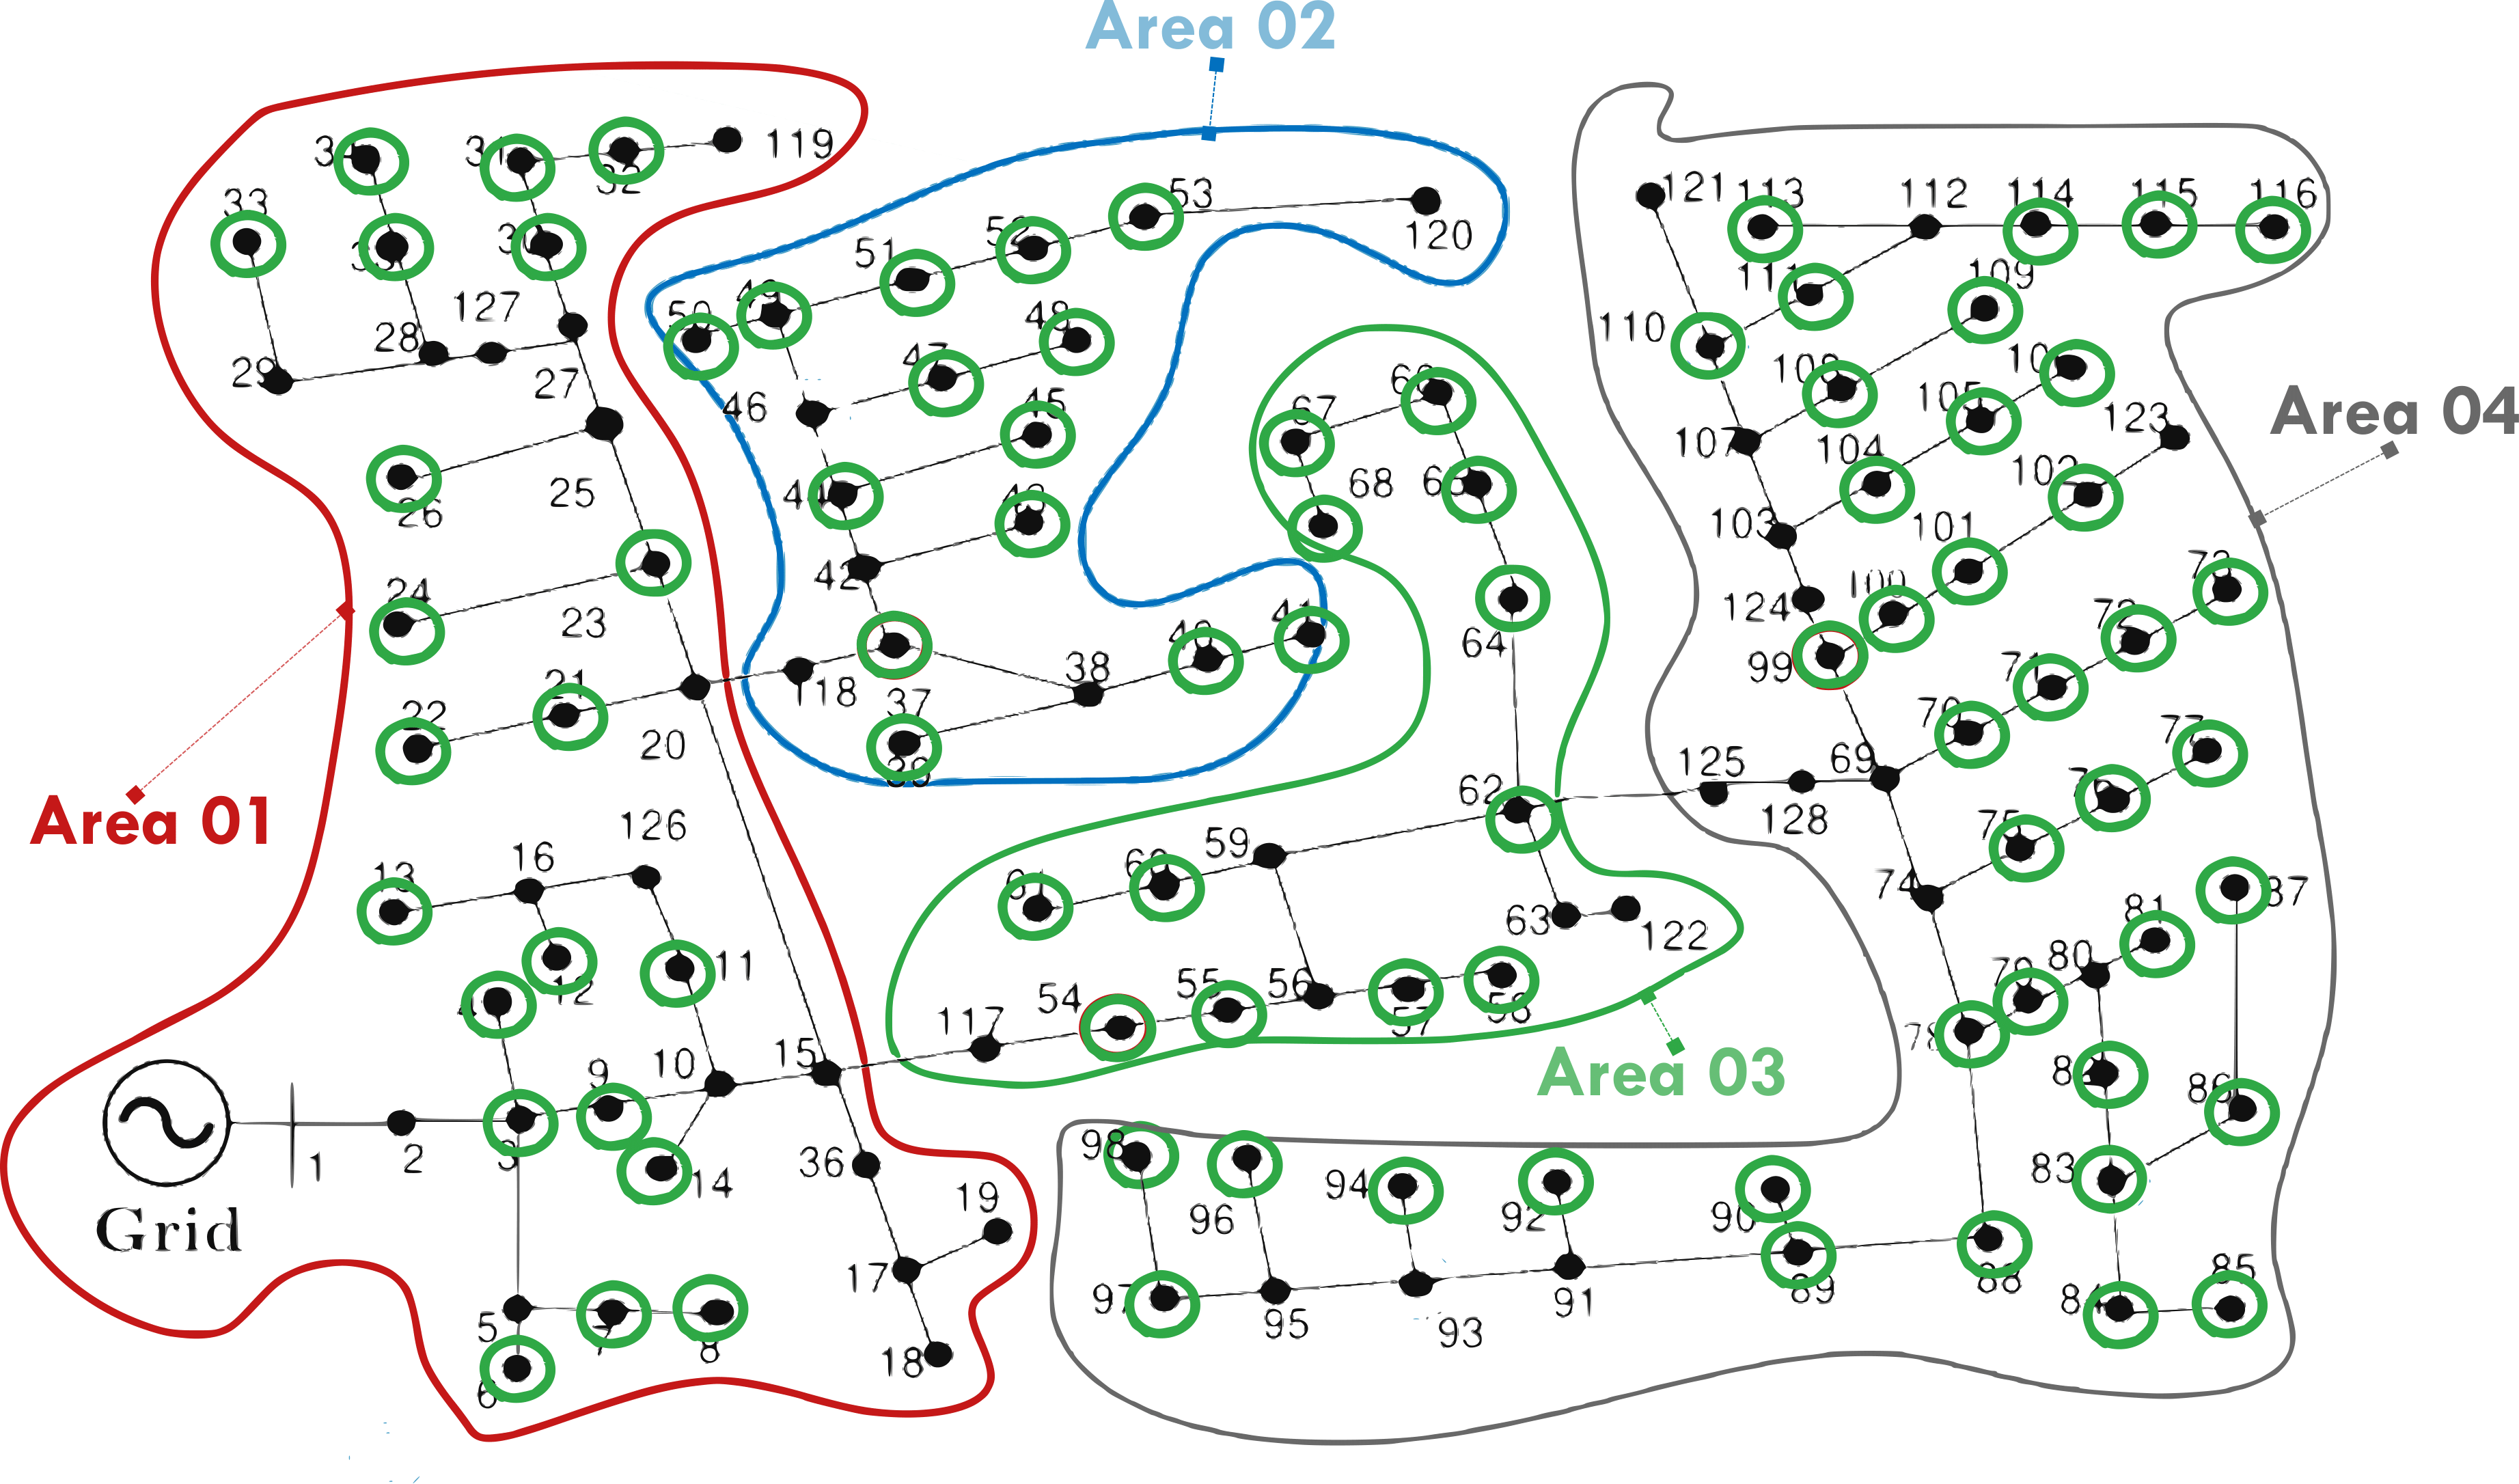
\includegraphics[width=\linewidth]{../figures/ieee123-FourAreas.png}
    \caption{IEEE 123 Node System Divided Into Four Areas}
    \label{fig:ieee123-four-area-figure}
\end{figure}


% \begin{figure}[h!]
%     \centering
%     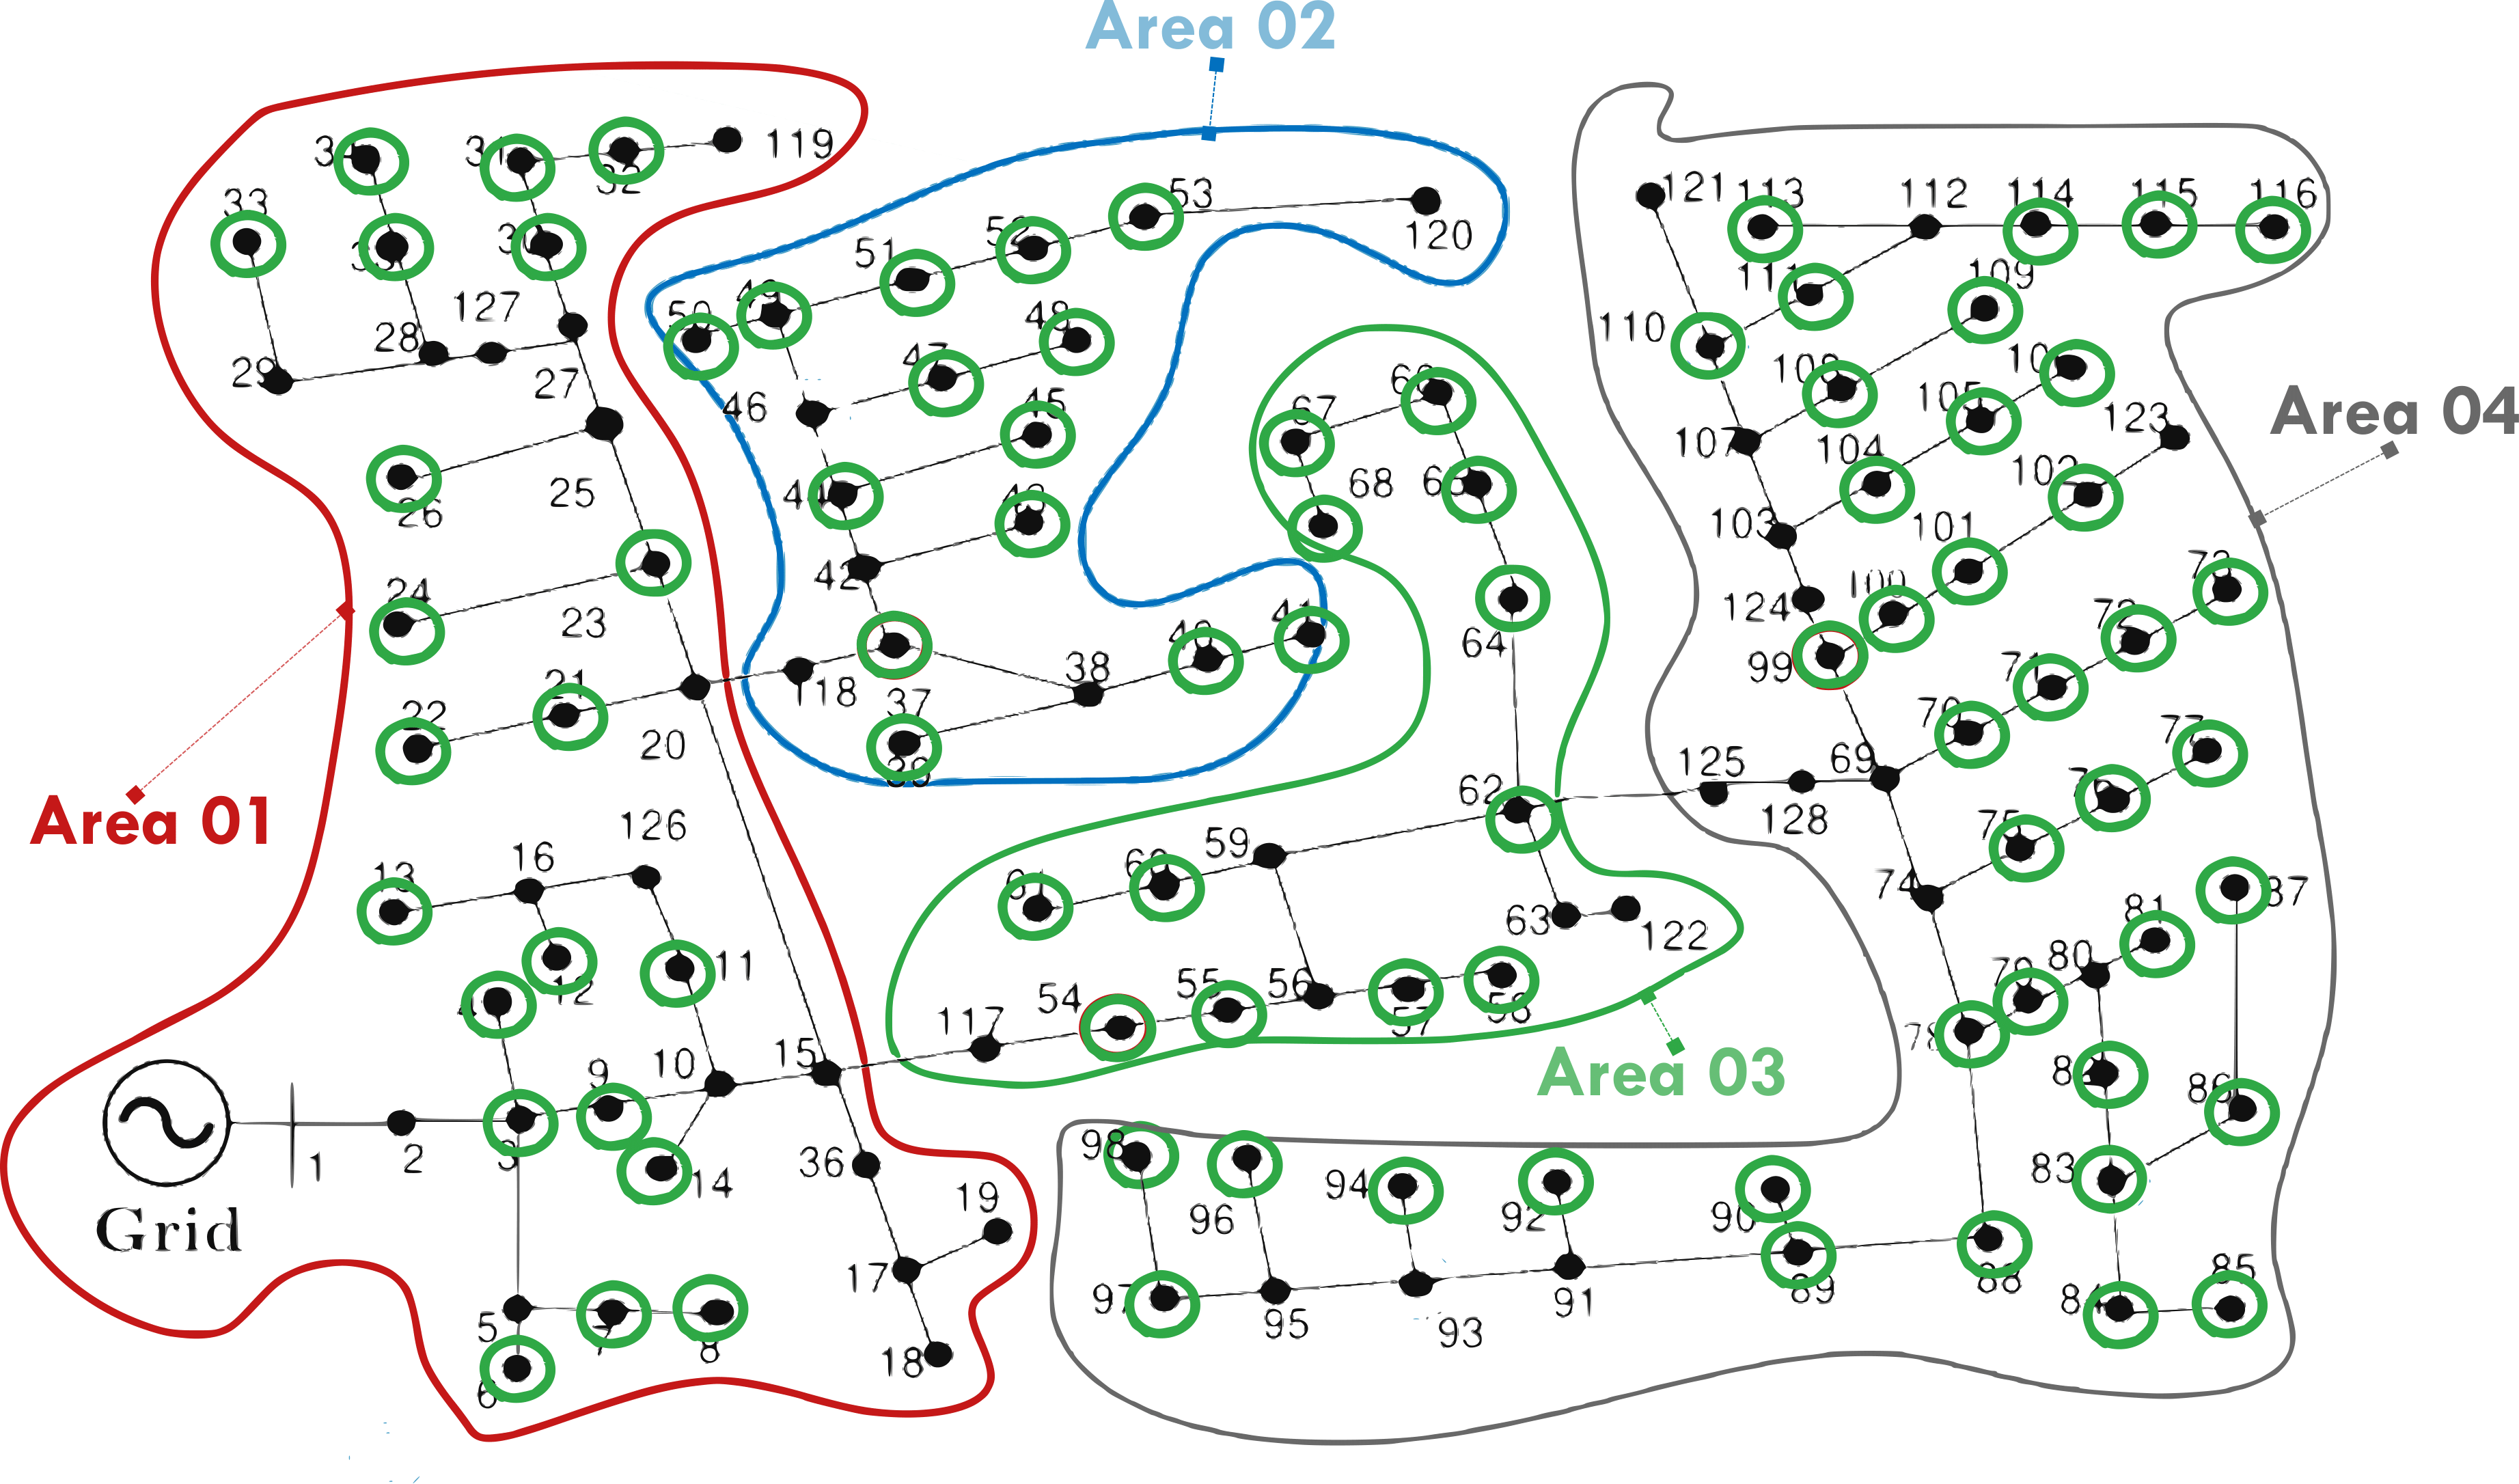
\includegraphics[width=\linewidth]{../figures/ieee123-FourAreas.png}
%     \caption{Input load and energy price data}
%     \label{fig:input_data}
% \end{figure}
\begin{figure}[h!]
    \centering
    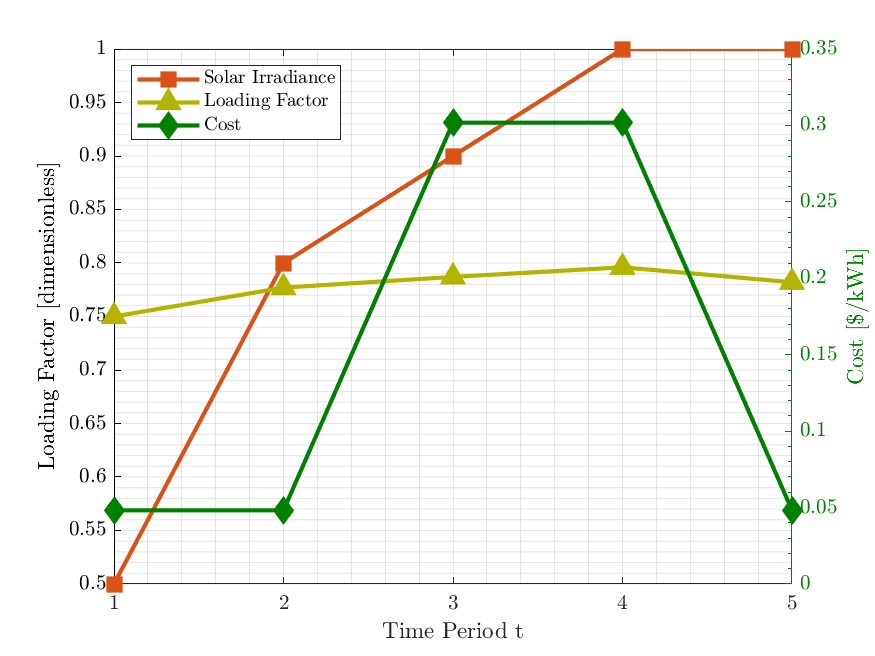
\includegraphics[height=0.25\textheight]{../figures/T5-inputCurves/InputCurves_Horizon_5.png}
    \caption{Time-series comparison for forecasts for Demand Power, Irradiance and Cost of Substation Power over a 5 Hour Horizon}
    \label{fig:inputCurve-5}
\end{figure}


\subsection{Simulation Results}
Case 1: centralized OPF with battery
Case 2: ENApp based distributed OPF with battery


\end{document}
